\section{Aufbau}

Der Aufbau, der schematisch in Abbildung \autoref{aufbau} dargestell ist, besteht aus einer Probe von einigen Millimetern Dicke zwischen den Platten eines Kondensators. Diese Probe wird über Heizwicklungen mit einem Heizstrom mit der gewünschten Rate erwämt. Da der Kristall hygroskopisch ist, befindet sich die Probe in einem zu allen Zeiten vakuumierten Rezipienten. Die Temperaturmessung erfolgt über ein an der Probe angeschlossenes Thermoelement. Für die Messung des Relaxationsstroms ist außerdem ein Pikoamperemeter vorhanden.
\begin{figure}
  \centering
  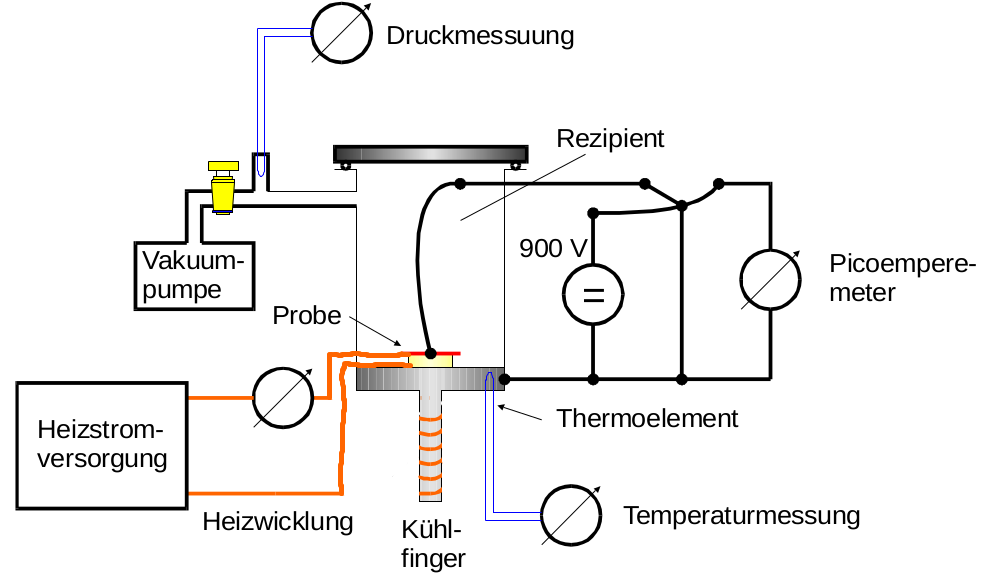
\includegraphics[width=0.75\textwidth]{img/aufbau.png}
  \caption{Schematischer Aufbau der Messapparatur \cite{FP}}
  \label{aufbau}
\end{figure}

\FloatBarrier

\section{Durchf\"{u}hrung}

Zunächst wird die Probe bei eingeschaltenem elektrischen Feld für ca. \SI{900}{\second} bis auf ungefähr \SI{320}{\kelvin} erwärmt. Dann wird der Heizstrom abgestellt und die Probe wird mit flüssigem Stickstoff auf etwa \SI{210}{\kelvin} abgekühlt. Das Feld an den Kondensatorplatten wird abgeschaltet und der Kondenstor kurzgeschlossen, um zu verhindern, dass Ladungsträger aus dieser Quelle die Messung des Relaxationsstroms stören. Nach einer Wartezeit von einigen Minuten wird das Pikoamperemeter angeschlossen und der Heizstrom so eingeregelt, dass eine konstante Heizrate von \SI{1.5}{\kelvin} bzw. \SI{2}{\kelvin} an der Probe gemessen wird. Sobald ein konstanter Strom gemessen wird, werden Wertepaare für die Temperatur und den Strom genommen.
